% !TEX root = morphkasten.tex

\section{Motor Lenkung}


%##############
\subsection{DC-Motor}

Im Kapitel 7.1 wurde die Variante DC-Motor bereits beschrieben.


%##############
\subsection{Schrittmotor}
Im Kapitel 7.2 wurde die Variante Schrittmotor bereits beschrieben.

%##############
\subsection{BLCD-Motor}
Im Kapitel 7.3 wurde die Variante BLCD-Motor bereits beschrieben.

%##############
\subsection{Servo-Motor}

\begin{figure}[h!]%Position festigen
\centering
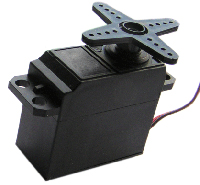
\includegraphics[width=0.5\textwidth]{fig/servo.jpg}
\caption{NiMH (Quelle: http://www.sachsendreier.com/asw/clernen/servo/servo.html)}
\label{fig:Java}
\end{figure}

\begin{table}[h]
\begin{tabular}{p{0.5\textwidth} | p{0.5\textwidth}}


 \textbf{Vorteile} & \textbf{Nachteile} \\ \hline
	 
\begin{itemize}
\item Sehr präzise
\item Sehr hoher Wirkungsgrad
\end{itemize}

 
 &
 
\begin{itemize}
\item Komplexe Ansteuerung
\item Hoher Anschaffungspreis
\item Hat einen begrenzten Drehwinkel
\item Relativ empfindlich
\end{itemize}

\end{tabular}
\end{table}

\begin{table}[h]
\begin{tabular}{p{0.5\textwidth}p{0.5\textwidth}}


 \textbf{Risiken} & \\ \hline
	 
\begin{itemize}
\item Erhötes Risiko das der Motor bei Versuchen Schaden nimmt.
\end{itemize}

 
\end{tabular}
\end{table}

\pagebreak